
\section{ISA Dataset Construction}

In this section, we introduce our ISA data collection and annotation process, as well as the related data analysis.

\subsection{Data Collection}


\begin{figure}[h]
    \centering
    \includegraphics[scale=0.5]{figs/samples3.pdf}
    \caption{Samples from the proposed ISA dataset. ES and SS stand for Entity Score and Semantic Score respectively.}
    % \KZ{The ERS and SRS seem to be defined on the scale of 1-5 but now they are a real number from 0 to 1. How do you scale them?}
    \label{samples}
\end{figure}


We collected our images from Pinterest\footnote{https://www.pinterest.com/}. 
% \KZ{Why Pinterest? Is there other possible soursces?}
% \XJ{There might be others, but currently we find pinterest good.}
After collecting images, we filtered out duplicated images using imagededup\footnote{https://github.com/idealo/imagededup}. 
To ensure high quality, we also manually excluded low-quality images that were blurry, watermarked or contained unnecessary text. 
% \KZ{Automatically or manually?}
After filtering, we finally retained 2,340 images in our dataset.


% We also filter out images with low quality. 

\subsection{Data Annotation}

For each image, we annotate it with two scores: an Entity Score and a Semantic Score. 
They correspond to the Entity Complexity Scoring task and the Semantic Complexity Scoring task, respectively.
% The range for each score is from 1 (Low) to 5 (High).
% The images are first annotated on a scale from 1 (Low) to 5 (High), after which the scores are normalized to [0,1] and the average is calculated as the final score.
For each score, the images are first annotated on a scale from 1 (Low) to 5 (High).
Then, these scores are normalized to the [0,1] range~\cite{ic9600}, and the average of these normalized scores is calculated as the final score.

\subsubsection{Entity Score}
The scoring criteria for the Entity Score are based on the richness of entities in the image.
Considering the importance of subjects like people and animals for semantic complexity, we have increased the weight of subject richness in the scoring.

The annotation criteria are shown in Figure~\ref{entity_ann}. 
Since we do not always expect images to be overly cluttered and overwhelming, a higher Entity Score does not necessarily indicate a better image.
% \MY{what does this mean?}

\begin{figure}[ht]
    \centering
    \includegraphics[scale=0.48]{figs/entity_ann2.pdf}
    \caption{Annotation criteria of Entity Score. The referenced Cookie Theft refers to the updated version.
    % \KZ{This pic takes too much space and not necessary. Instead of showing this pic, you can show what you mean by few, and what you mean by abundant. These words are very vague. Maybe Fig 4 will help. But you gotta make sure that annotators get clear instruction about the definitions of these 5 levels.}
    }
    \label{entity_ann}
\end{figure}

\subsubsection{Semantic Score}

In order to help annotators understand the meaning of semantic complexity, we construct detailed annotation criteria of Semantic Score (Figure~\ref{semantic_ann}).
The scoring criteria mainly consist of five dimensions: event, connection between events, visual clues, storytelling, and interest level of the story.
The connection between events primarily refers to the causal relationship between events.
For instance, because ``there's a broken bowl on the floor,''  ($\rightarrow$) ``the mother is spanking the boy.''
% \MY{use an arrow to suggest the causal relations? such a sentence is less effective in expressing what you mean.}
The definition of visual clues is entities capable of inferring new semantic conclusions. 
% For example, a ``Christmas tree'' is a visual clue for inferring Christmas\MY{``for time reasoning, as it suggests Christmas season''}.
For example, a ``Christmas tree'' is a visual clue for time reasoning, as it suggests the Christmas season.

Specifically, the interpretation of Figure~\ref{semantic_ann} is as follows:
(1). If there is no event happening in the image, or if there is only a single kind of event (e.g., running, swimming, etc.), give it a score of 1.
(2). If there is one or more kinds of events in the image, but the events are unrelated and there are almost no clues to infer additional information, give it a score of 2.
(3). Assign a score of 2 when there is one or more events in the image with a slight connection between them or a few clues that suggest additional information, but the image does not convey a clear story or the story's appeal is minimal.
(4). For images rated 3 or above, there must be connections between events and visual clues present in the image. 
(5). The differences between ratings of 3, 4, and 5 primarily lie in the richness and number of these connections and clues.
% \MY{can we have a table summarizing these rules? or combine with fig.2 for entity.}
% \XJ{This is the interpretation of Figure~\ref{semantic_ann}, maybe keep it as a paragraph?}


\subsubsection{Annotation Process}
For each image, three annotators are hired to annotate the two scores.
The annotators are mostly undergraduate and graduate students aged 20 to 25.
% \MY{be specific about the background, age of these annotators}
We first provided training for the annotators. 
For each annotation score, several examples are provided for the annotators to refer to. 
They were then asked to perform annotation on a small sample set of data as a test first. 
% Only after the trial annotations met the standards did we proceed with the formal annotation process.
Only annotators who pass the test are allowed to participate in the subsequent formal annotation.

% During annotation, we kept randomly sample annotation results and provided feedback to annotators to help them imporve annotation accuracy. 
During the annotation process, we randomly sample the annotated data and provide timely feedback to the annotators to further help them improve labeling quality.
% \MY{to ensure label quality? since subjective annotation is difficult to define accuracy}.
We also provide immediate assistance if they encounter any issues during the annotation process.
If a sample from a particular group of images has poor annotation results, we will discard the labels for that group and re-label the group of images.
% \KZ{This para is not clear.}

% Then, we calculate a final score ...
%Following~\citet{ic9600}, the final Entity Score or Semantic Score is acquired by averaging the 3 labels and is then normalized to [0,1] with the formula $s_j = \sum_{i=1}^3\left(y_j^i-1\right) / (4\times3)$, where $y^i_j \in [1, 2, 3, 4, 5]$ and is the $i$th label of the $j$th sample.


% \begin{table*}[h]
%     \centering
%     %\resizebox{.95\columnwidth}{!}{
%     \begin{tabular}{l|ccccc}
%     \toprule
%     Score & Event  &  Connection between the entities &  Visual clues &  Storytelling & Interest level of the story
%     \\
%     \midrule 
%       & 0.182 & 0.378 & 0.626 & 0.614 \\
%     ViT & 0 & 0 & 0 & 0  \\
%     ViLT & 0 & 0 & 0 & 0  \\
%     GPT-4o + BERT & 0 & 0 & 0 & 0  \\
%     GPT-4o + Longformer & 0 & 0 & 0 & 0  \\
%     \bottomrule
% \end{tabular}
% \caption{Semantic Score.}
% \label{table2}
% \end{table*}

\begin{figure*}[htbp]
    \centering
    \includegraphics[scale=0.55]{figs/semantic_ann2.pdf}
    \caption{Annotation criteria of Semantic Score.}
    \label{semantic_ann}
\end{figure*}





\subsection{Dataset Analysis}



\subsubsection{Annotation Consistency}

In line with established standards~\cite{kong2016photo, ying2020patches, ic9600}, we assess the consistency between annotators by using the Pearson Correlation Coefficient (PCC), Spearman's Rank Correlation Coefficient (SRCC), and Kendall's tau correlation for each pair of annotations.
% and evaluate their statistical significance of the correlation with respect to a null hypothesis of uncorrelated responses. 
For Entity Score, the average PCC, SRCC, and Kendall's tau are 0.813, 0.803, and 0.760 respectively.
The average PCC, SRCC, and Kendall's tau of Semantic Score are 0.773, 0.773, and 0.707 respectively.
This demonstrates the consistency of our data annotation.

% Besides, similar to the crowdsourcing assessment studies for IQA, IAA and ICA~\cite{koniq10k, Siahaan2016, ic9600}, we calculate the intra-class correlation coefficient (ICC) of our annotation. 
In addition, similar to the crowdsourcing assessment studies conducted for IQA, IAA, and ICA~\cite{koniq10k, Siahaan2016, ic9600}, we compute the Intra-class Correlation Coefficient (ICC) for our annotations to measure the inter-rater reliability.
Same as~\citet{koniq10k, Siahaan2016, ic9600}, we adopt the same one way random model of ICC. 
The ICCs of Entity Score and Semantic Score are 0.926 and 0.909 respectively, which shows the reliability and consistency of our annotation.

% {'Entity Pearson': 0.8127308825110332,
%  'Entity Spearman': 0.8031187977664768,
%  'Entity Kendall_tau': 0.7599569314943596,
%  'Semantic Pearson': 0.7729549059162825,
%  'Semantic Spearman': 0.7725143494872039,
%  'Semantic Kendall_tau': 0.7066790164804804}


\subsubsection{Dataset Case Analysis}

Figure~\ref{samples} shows some samples of our dataset. 
% \KZ{Explain the scores in the figures, why they are in [0, 1]?}
% \XJ{It is introduced in Annotation Process section.}
We can see that images with more entities are scored with higher Entity Scores, and images with more visual clues and telling more engaging stories are scored with higher Semantic Scores.
We can also see that the relationship between Entity Score and Semantic Score is not entirely positively correlated.
Even though some images contain few entities, for example, Figure~\ref{samples} (e), they can still tell an interesting story.
Images with a variety of entities can also contain little semantic information, for instance, Figure~\ref{samples} (d). 

\subsubsection{Dataset Statistics}

Table~\ref{distribution} shows the distribution of our dataset.
We randomly split the data into a training set and a test set in a 7:3 ratio.

% \begin{figure}[H]
%     \centering
%     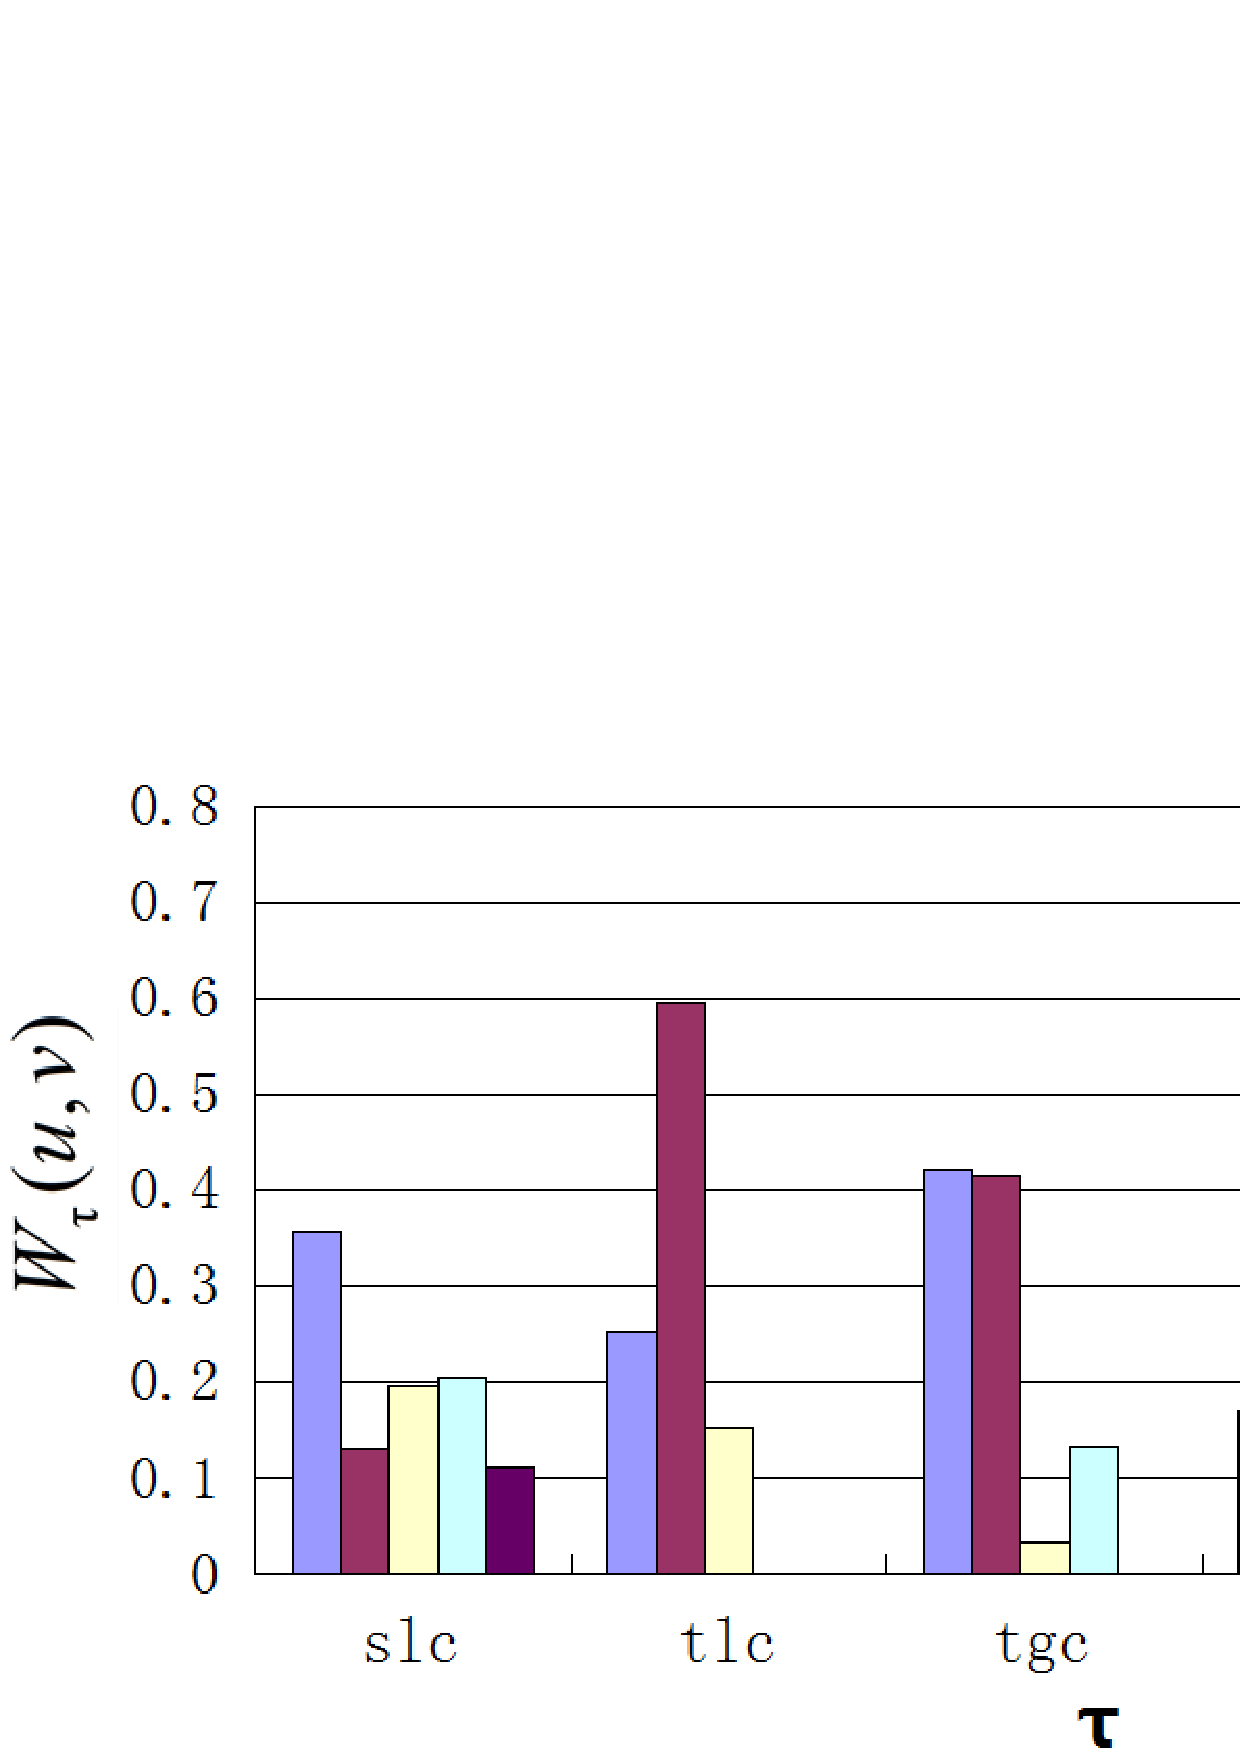
\includegraphics[scale=0.5]{figs/distribution.pdf}
%     \caption{Dataset label distribution.\MY{still use 1-5 on x-axis might be easier to understand. or you can actually use a table to show this? the fig is taking up a a lot of space and make the differences very obvious}}
%     \label{distribution}
% \end{figure}


% \begin{figure}[H]
%     \centering
%     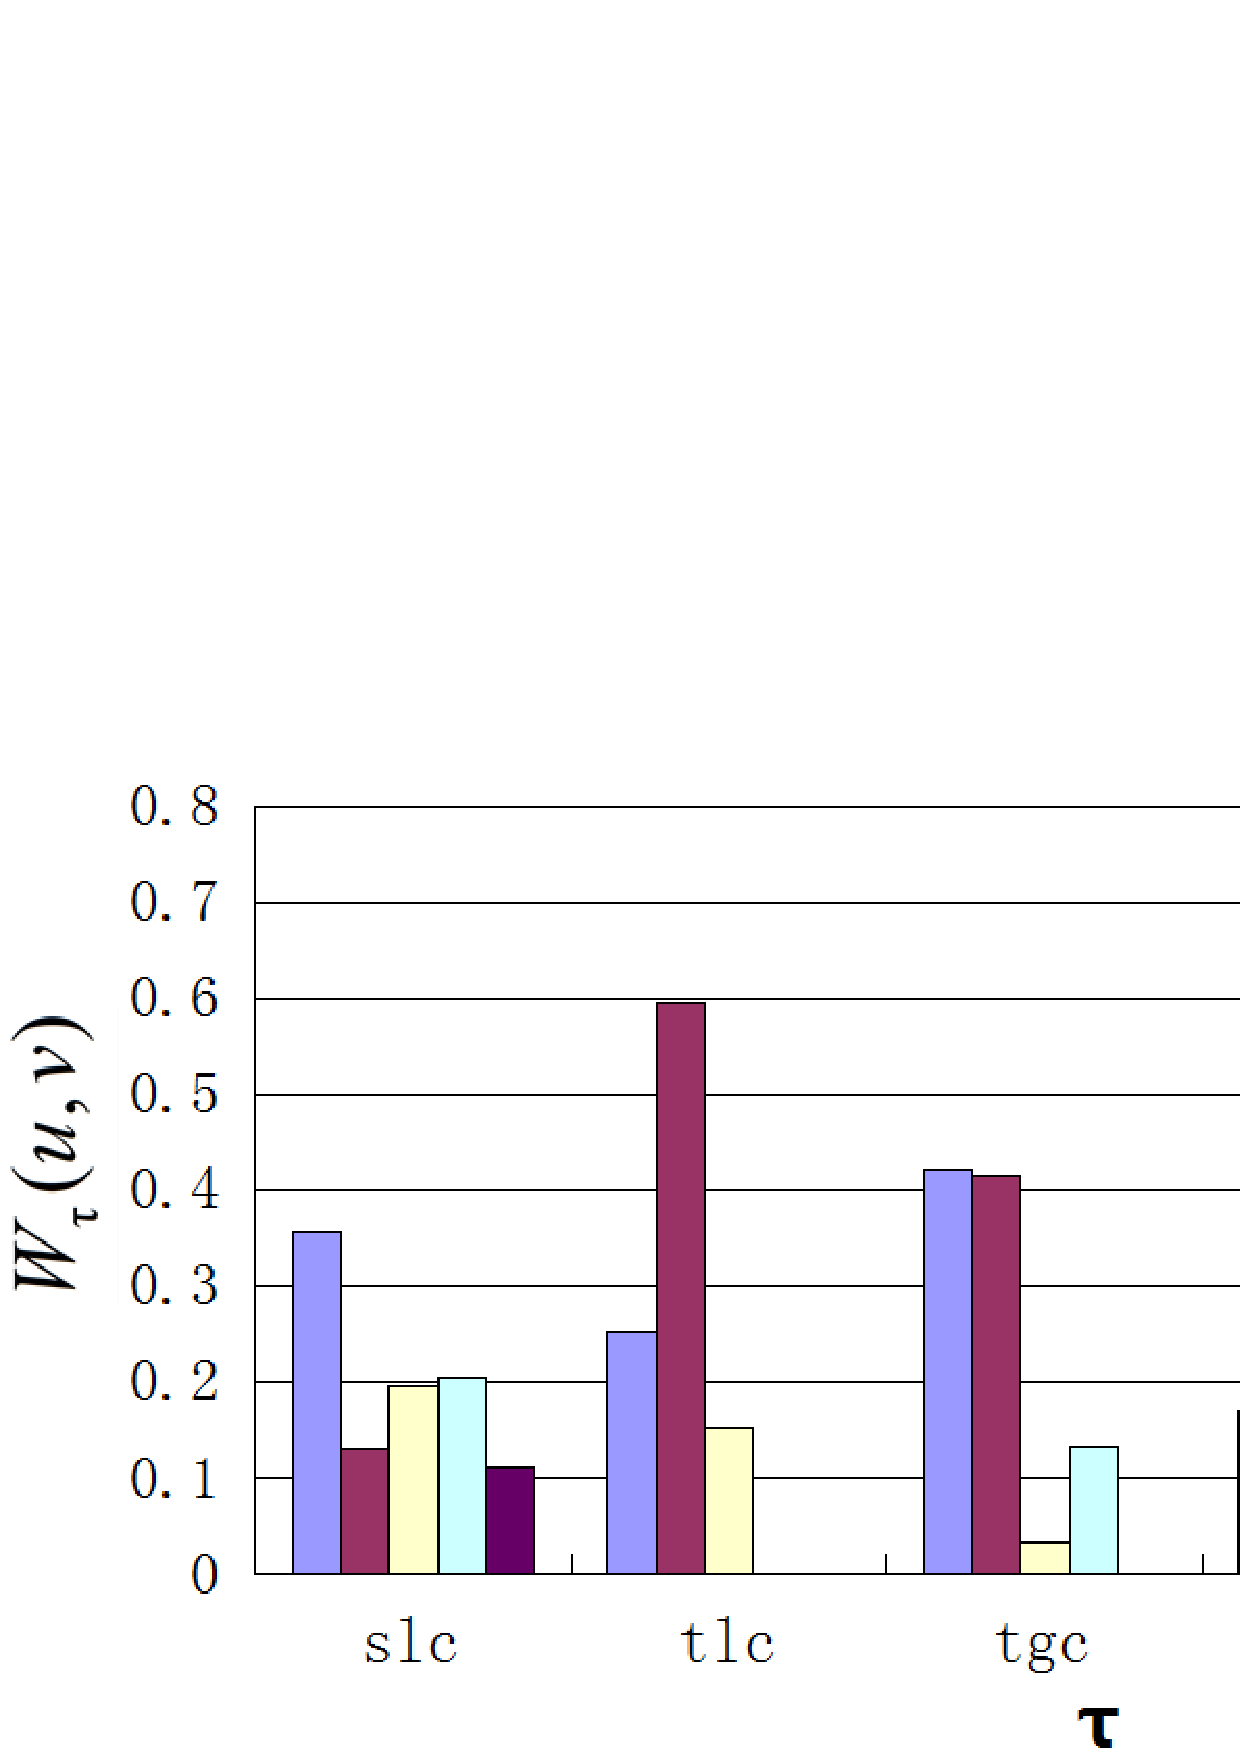
\includegraphics[scale=0.5]{figs/distribution.pdf}
%     \caption{Dataset label distribution.\MY{still use 1-5 on x-axis might be easier to understand. or you can actually use a table to show this? the fig is taking up a a lot of space and make the differences very obvious}}
%     \label{distribution}
% \end{figure}


\begin{table}[h]
    \centering
    \resizebox{.95\columnwidth}{!}{
    \begin{tabular}{l|ccccc}
    \toprule
    Score & [0, 0.2) & [0.2, 0.4) & [0.4, 0.6) & [0.6, 0.8) & [0.8, 1]\\
    \midrule 
    ES & 445 & 834 & 869 & 118 & 74 \\
    SS & 549 & 670 & 777 & 273 & 71 \\
    \bottomrule
\end{tabular}}
\caption{Dataset label distribution. ES and SS stand for Entity Score and Semantic Score respectively.}
\label{distribution}
\end{table}

